\documentclass[%
 aip,
 amsmath,amssymb,
 reprint,%
]{revtex4-2}

\usepackage{graphicx}% Include figure files
\usepackage{dcolumn}% Align table columns on decimal point
\usepackage{bm}% bold math
\usepackage[utf8]{inputenc}
\usepackage[T1]{fontenc}
\usepackage{etoolbox}
\usepackage{booktabs}
\usepackage{hyperref}
\usepackage{xcolor}
\usepackage{amsthm}

\DeclareMathAlphabet{\mathscr}{OMS}{cmsy}{m}{n}

\newcommand{\RLs}{\mathcal{R}_L^{\mathrm{stat}}}
\newcommand{\RLd}{\mathcal{R}_L^{\mathrm{diff}}}

\makeatletter
\def\@email#1#2{%
 \endgroup
 \patchcmd{\titleblock@produce}
  {\frontmatter@RRAPformat}
  {\frontmatter@RRAPformat{\produce@RRAP{*#1\href{mailto:#2}{#2}}}\frontmatter@RRAPformat}
  {}{}
}%
\makeatother

\newtheorem{proposition}{Proposition}
\newtheorem{theorem}{Theorem}
\newtheorem{definition}{Definition}

\begin{document}

\title{The Landauer Saturation Diagnostic for Non-Gravitational Systems:\\
QCD Confinement and the Casimir Effect}

\author{Moses Rahnama}
\email{moses@minaanalytics.com}
\affiliation{Mina Analytics, New York, United States}

\date{\today}

\begin{abstract}
We define the static Landauer ratio
$\RLs \equiv U/(T S)$, which equals the Euler homogeneity
degree of the entropy with respect to energy when $S(U)$ is a
homogeneous function, and compute it for
two non-gravitational systems
with complete thermodynamic decompositions.
For QCD static-quark thermodynamics, using lattice data from
Kaczmarek and Zantow ($N_f = 2$, $T_c = 200$~MeV), we find
$\RLs > 1$ at all sampled temperatures
($0.79 \leq T/T_c \leq 2.99$), with a minimum
$\RLs \approx 1.17$ at the deconfinement transition and
$\RLs \approx 2.16$ in deep confinement; the ratio crosses
unity only at $T/T_c \gtrsim 3$ and vanishes at asymptotically
high temperatures by asymptotic freedom.
Continuum-extrapolated (2+1)-flavor data from Bazavov et
al.\ confirm this qualitative pattern with physical quark masses.
We conjecture that $\RLs > 1$ in the confined phase ($T < T_c$)
is a generic thermodynamic signature of confinement in
asymptotically free gauge theories.
For the thermal Casimir effect between perfect conductors, the
high-temperature limit gives $\RLs \to 0$ (purely entropic
free energy).
Applying the same definition to gravitational systems, the
Schwarzschild black hole gives $\RLs = 2$ exactly
(via the Smarr relation $Mc^2 = 2\,T_H S_{BH}$), while the
cosmological apparent horizon gives $\RLs = 1$ (via the
Misner--Sharp energy $E_{MS} = T_{\mathrm{GH}} S$; this value depends on the
quasi-local energy definition~\cite{Trivedi2024}).
Together with the photon gas ($\RLs = 3/4$, exact from
Stefan--Boltzmann), these results define a three-regime
classification: super-Landauer ($\RLs > 1$, black holes and
QCD confinement), statically saturating ($\RLs = 1$,
cosmological apparent horizon in Misner--Sharp accounting;
note that Paper~C's \emph{differential} ratio gives
$\RLd = 1/2$ for this system), and sub-Landauer ($\RLs < 1$,
referring to the static energy-to-information ratio, not to
erasure-bound violations; photon gas, high-temperature Casimir).
We note that geometric scaling of information stored on a
$d$-dimensional manifold yields a force $F \sim r^{d-1}$ for
$d \geq 1$ (or $F \sim 1/r^2$ for point sources, $d = 0$),
which the Landauer framing interprets thermodynamically but does not
derive.
Numerical claims from the Kaczmarek--Zantow dataset and derived
quantities are verified by a companion simulation with
80 falsifiable checks across 9 groups.
\end{abstract}

\maketitle

% ============================================================
\section{Introduction}

Landauer's principle~\cite{Landauer1961} sets a thermodynamic floor
on the cost of erasing one bit of information: $Q \geq k_B T \ln 2$.
Cort\^es and Liddle~\cite{Cortes2024} showed that Hawking evaporation
saturates this bound: each bit of Bekenstein--Hawking entropy lost
during black hole evaporation releases exactly $k_B T_H \ln 2$ of
energy.

In Paper~C~\cite{Rahnama2026BlackHole} we formalized this observation
through a \emph{differential} Landauer saturation ratio
$\mathcal{R}_L^{\mathrm{diff}} = \delta E / (T\,\delta S)$, which
measures the energy cost per bit during a thermodynamic process.
Schwarzschild black holes give
$\mathcal{R}_L^{\mathrm{diff}} = 1$ (from $dM = T_H\,dS_{BH}$),
while Trivedi's quasi-local accounting at the cosmological apparent
horizon gives
$\mathcal{R}_L^{\mathrm{diff}} = 1/2$~\cite{Trivedi2024}.

For static systems in thermal equilibrium, the differential ratio
is uninformative: the first law $dU = T\,dS$ (at fixed volume)
gives $\mathcal{R}_L^{\mathrm{diff}} = 1$ for any equilibrium
system.  A more useful diagnostic for static systems is the
\emph{static Landauer ratio}
\begin{equation}
\RLs \;\equiv\; \frac{U}{T\,S},
\end{equation}
which compares the total internal energy to the total
entropy-weighted temperature.  For any system obeying
$\partial S/\partial U = 1/T$, if the entropy is a homogeneous
function of internal energy of degree~$n$ (at fixed extensive
variables), Euler's theorem gives $U\,\partial S/\partial U = n\,S$,
i.e.\ $U/T = n\,S$, so $U = n\,T\,S$ and
$\mathcal{R}_L^{\mathrm{stat}} = n$.  The static ratio is therefore
the Euler homogeneity degree of the entropy with respect to
energy~\cite{Callen1985,KastorRayTraschen2009}.  We adopt the name
``Landauer ratio''
because $T\,S = N_{\mathrm{bits}}\,k_B T \ln 2$ equals the total
Landauer maintenance cost of the system's information content, but
the diagnostic itself is a standard thermodynamic quantity whose
value can be read off from the equation of state without invoking
information theory.  (Throughout, $\RLs = U/(TS)$ is
convention-invariant: its numerical value is independent of whether
entropy carries explicit $k_B$ factors.  In the QCD lattice
sections, $S_\infty$ is dimensionless (natural units); in the
black hole sections, $S_{BH}$ carries $k_B$.  The ratio $U/(TS)$
is the same either way.)

Applied to gravitational systems, the static ratio gives different
values from the differential one.  For a Schwarzschild black hole,
the Smarr relation~\cite{Smarr1973}
$Mc^2 = 2\,T_H S_{BH}$ gives
\begin{equation}
\label{eq:RL_BH}
\mathcal{R}_L^{\mathrm{BH}} = \frac{Mc^2}{T_H\,S_{BH}} = 2.
\end{equation}
For the cosmological apparent horizon, adopting the Misner--Sharp
quasi-local energy $E_{MS}$ and the Gibbons--Hawking temperature
gives $E_{MS} = T_{\mathrm{GH}}\,S$, hence
$\mathcal{R}_L^{\mathrm{cosmo}} = 1$; this value depends on the
choice of quasi-local energy definition (see
Trivedi~\cite{Trivedi2024} for the underlying accounting).

Here we compute $\RLs$ for two non-gravitational
systems where complete thermodynamic decompositions (free energy,
internal energy, entropy) are available from first principles or
lattice data:
\begin{enumerate}
\item \textbf{QCD static-quark thermodynamics}: the free energy,
internal energy, and entropy of a static quark--antiquark pair
(connected by a chromoelectric flux tube below $T_c$, color-screened
above $T_c$), studied on the lattice by Kaczmarek and
Zantow~\cite{KZ2005a,KZ2005b}.
\item \textbf{Thermal Casimir effect}: the vacuum fluctuation force
between perfectly conducting plates at finite
temperature~\cite{Casimir1948,Lifshitz1956}.
\end{enumerate}

The paper is organized as follows.
Section~\ref{sec:storage_dim} recalls the geometric-scaling
correspondence between storage dimension and force law.
Section~\ref{sec:qcd} applies $\mathcal{R}_L^{\mathrm{stat}}$ to
QCD static-quark thermodynamics.
Section~\ref{sec:casimir} treats the thermal Casimir effect.
Section~\ref{sec:classification} presents the unified classification.
Section~\ref{sec:perturbative} analyzes the perturbative high-$T$
limit.
Section~\ref{sec:scope} states what we do and do not claim.
Section~\ref{sec:conclusion} concludes.


% ============================================================
\section{Storage-dimension observation}
\label{sec:storage_dim}

The relationship between the dimensionality of information storage
and the resulting force law follows from geometric scaling.
If information is stored uniformly on a $d$-dimensional structure
of characteristic scale~$r$, the total information content scales
as $N \sim r^d$.  Because the thermodynamic maintenance potential
$\Phi$ is proportional to $N$, we have $\Phi \sim r^d$ for
$d \geq 1$, yielding a radial force
$F = -d\Phi/dr \sim r^{d-1}$.

For unconfined, localized information ($d = 0$), the bits are
broadcast outward.  The field energy density required to maintain
this configuration scales as $u \sim 1/r^4$ (as in Coulomb or
Newtonian fields); integrating the field energy outside radius~$r$
gives $\Phi(r) = \int_r^{\infty} u\,4\pi r'^2\,dr' \sim 1/r$
and an inverse-square force $F \sim 1/r^2$.

Table~\ref{tab:storage_dim} collects the correspondence.
The Landauer framing provides a thermodynamic interpretation for
these potentials (the maintenance cost per bit is $k_B T \ln 2$).
For $d \geq 1$ the force-law exponents are fixed entirely by the
geometry of the storage manifold.  The $d = 0$ case additionally
requires the field energy density $u \sim 1/r^4$ as input
(a dynamical fact about the underlying field theory), yielding
the inverse-square law.
$d = 1$ gives a constant force (QCD confinement), and $d = 2$ gives
a linear restoring force.

\begin{table}[b]
\centering
\caption{Storage dimension and force law from geometric scaling.}
\label{tab:storage_dim}
\begin{tabular}{@{}clll@{}}
\toprule
$d$ & Storage geometry & $\Phi(r)$ & Force law \\
\midrule
0 & Point (broadcast) & $\sim 1/r$ & $\sim 1/r^2$ \\
1 & Line (flux tube)  & $\sim r$   & $\sim$ const \\
2 & Surface           & $\sim r^2$ & $\sim r$ \\
\bottomrule
\end{tabular}
\end{table}


% ============================================================
\section{QCD static-quark thermodynamics: \texorpdfstring{$\RLs$}{RL-stat} from lattice data}
\label{sec:qcd}

\subsection{Setup}

The free energy $F_{\infty}(T)$, internal energy $U_{\infty}(T)$,
and entropy $S_{\infty}(T)$ of a static quark--antiquark pair at
infinite separation have been computed on the lattice by Kaczmarek and
Zantow~\cite{KZ2005a,KZ2005b} for $N_f = 2$ QCD with
$T_c = 200$~MeV.  These quantities satisfy
\begin{equation}
F_{\infty}(T) = U_{\infty}(T) - T\,S_{\infty}(T).
\end{equation}

The static Landauer ratio for this system is
\begin{equation}
\label{eq:RL_qcd}
\mathcal{R}_L^{\mathrm{QCD}}(T) = \frac{U_{\infty}(T)}{T\,S_{\infty}(T)}.
\end{equation}

\subsection{Lattice data}

We use the data from Table~I of Ref.~\cite{KZ2005a}:
$S_{\infty}(T)$ (dimensionless) and $U_{\infty}(T)/T_c$
(dimensionless) at 16 temperatures spanning $0.79 \leq T/T_c \leq 2.99$.
Table~\ref{tab:qcd_rl} presents the computed $\RLs$.
The $F_{\infty}/T_c$ column is not independent data; it is computed
from $F_{\infty} = U_{\infty} - T\,S_{\infty}$.

\begin{table}[t]
\centering
\caption{Static Landauer ratio for the QCD static $q\bar{q}$ system.
Data from Kaczmarek and Zantow~\cite{KZ2005a}, $N_f = 2$,
$T_c = 200$~MeV.  $N_{\mathrm{bits}} = S_{\infty}/\ln 2$.
Points with $T/T_c > 1$ are in the deconfined (color-screened)
regime; the system is a flux tube only for $T < T_c$.}
\label{tab:qcd_rl}
\begin{tabular}{@{}rrrrrr@{}}
\toprule
$T/T_c$ & $S_{\infty}$ & $U_{\infty}/T_c$ & $N_{\mathrm{bits}}$ &
$F_{\infty}/T_c$ & $\RLs$ \\
\midrule
0.79 &  5.48 &  9.37 &  7.91 & 5.04 & 2.164 \\
0.84 &  6.49 & 10.19 &  9.36 & 4.74 & 1.868 \\
0.88 &  7.78 & 11.30 & 11.22 & 4.45 & 1.650 \\
0.93 & 12.92 & 15.96 & 18.64 & 3.94 & 1.328 \\
0.98 & 16.38 & 19.27 & 23.63 & 3.22 & 1.200 \\
1.01 & 14.83 & 17.71 & 21.39 & 2.73 & 1.183 \\
1.04 & 12.93 & 15.78 & 18.65 & 2.33 & 1.173 \\
1.09 &  5.49 &  7.84 &  7.92 & 1.86 & 1.310 \\
1.13 &  3.95 &  6.14 &  5.70 & 1.67 & 1.375 \\
1.19 &  2.73 &  4.72 &  3.94 & 1.47 & 1.453 \\
1.29 &  1.63 &  3.37 &  2.35 & 1.27 & 1.603 \\
1.43 &  1.25 &  2.85 &  1.80 & 1.06 & 1.594 \\
1.57 &  1.02 &  2.51 &  1.47 & 0.91 & 1.567 \\
1.72 &  0.91 &  2.32 &  1.31 & 0.76 & 1.483 \\
1.89 &  0.87 &  2.26 &  1.26 & 0.62 & 1.375 \\
2.99 &  0.67 &  2.09 &  0.97 & 0.09 & 1.043 \\
\bottomrule
\end{tabular}
\end{table}

\subsection{Results}

Figure~\ref{fig:rl_qcd} plots $\RLs(T/T_c)$.
Three features stand out:

\begin{enumerate}
\item \textbf{$\RLs > 1$ at all sampled temperatures.}
At all 16 data points ($0.79 \leq T/T_c \leq 2.99$), the
internal energy exceeds $TS$ (i.e., $U > TS$).  The static
$q\bar{q}$ system is \emph{super-Landauer} throughout this
range, including points well into the deconfined regime.
As shown in Section~\ref{sec:perturbative}, $\RLs$ crosses
unity at $T/T_c \gtrsim 3$ and vanishes asymptotically.

\item \textbf{Minimum at $T_c$.}
$\RLs$ reaches its minimum value $\approx 1.17$ at
$T/T_c \approx 1.04$, coinciding with the deconfinement phase
transition.  The entropy also peaks near $T_c$
($N_{\mathrm{bits}} \approx 23.6$ at $T/T_c = 0.98$), reflecting the
maximal liberation of color degrees of freedom.

\item \textbf{Deep confinement approaches the black hole value.}
At $T/T_c = 0.79$, $\RLs \approx 2.16$.  This is within $\sim 8\%$
of the Schwarzschild value $\RLs = 2$ (Eq.~\ref{eq:RL_BH}).
The BH value is exact (from holographic scaling), while the QCD value
is a lattice result at $N_f = 2$ with heavier-than-physical pion
masses~\cite{KZ2005a}, so the numerical proximity should
be treated with caution.
Nonetheless, both systems share the structural feature of confining
information behind a boundary.
\end{enumerate}

To test robustness beyond the $N_f = 2$ dataset, we compute
$\RLs$ from the continuum-extrapolated (2+1)-flavor data of
Bazavov et al.~\cite{Bazavov2016}, who report the single-quark
free energy $F_Q(T)$ and entropy $S_Q(T) = -\partial F_Q/\partial T$
with physical quark masses and $T_c \approx 155$~MeV.  The
single-quark internal energy is $U_Q = F_Q + T\,S_Q$, and the
ratio $\RLs = U_Q/(T\,S_Q)$ is identical to the pair ratio
because going from $F_Q$ to $F_\infty = 2F_Q$ doubles both
$U_\infty$ and $S_\infty$ (by cluster decomposition), leaving
$\RLs$ invariant.

Table~\ref{tab:bazavov_rl} shows the result at representative
temperatures.  The qualitative pattern matches the $N_f = 2$ data:
$\RLs > 1$ throughout the confined and near-$T_c$ region, with a
minimum $\RLs \approx 1.68$ at $T/T_c \approx 1.03$, rising to
$\RLs \approx 2.93$ in deep confinement.  The crossing
$\RLs = 1$ occurs at $T \approx 450$~MeV ($T/T_c \approx 2.9$),
consistent with the $N_f = 2$ estimate ($T/T_c \gtrsim 3$).

The quantitative values differ from the $N_f = 2$ results
(e.g., minimum $\RLs \approx 1.68$ vs.\ $1.17$), reflecting the
different renormalization conventions for $F_Q$ and different
lattice setups.  Crucially, both datasets agree on the
qualitative pattern: super-Landauer in confinement, minimum at
$T_c$, and crossing to sub-Landauer above $T/T_c \sim 3$.

\begin{table}[b]
\centering
\caption{Static Landauer ratio from Bazavov et al.\ (2+1)-flavor
continuum-extrapolated data~\cite{Bazavov2016},
$T_c = 155$~MeV.  $U_Q = F_Q + T\,S_Q$.}
\label{tab:bazavov_rl}
\begin{tabular}{@{}rrrrrr@{}}
\toprule
$T$~[MeV] & $T/T_c$ & $F_Q$~[MeV] & $S_Q$ & $U_Q$~[MeV] & $\RLs$ \\
\midrule
125 & 0.81 &  481 & 1.99 &  730 & 2.93 \\
140 & 0.90 &  446 & 2.78 &  835 & 2.15 \\
155 & 1.00 &  395 & 3.67 &  964 & 1.69 \\
160 & 1.03 &  377 & 3.47 &  932 & 1.68 \\
200 & 1.29 &  268 & 2.15 &  698 & 1.62 \\
300 & 1.94 &  121 & 1.07 &  442 & 1.38 \\
400 & 2.58 &   34 & 0.75 &  334 & 1.11 \\
500 & 3.23 & $-32$ & 0.60 &  268 & 0.89 \\
\bottomrule
\end{tabular}
\end{table}

\begin{figure}[t]
\centering
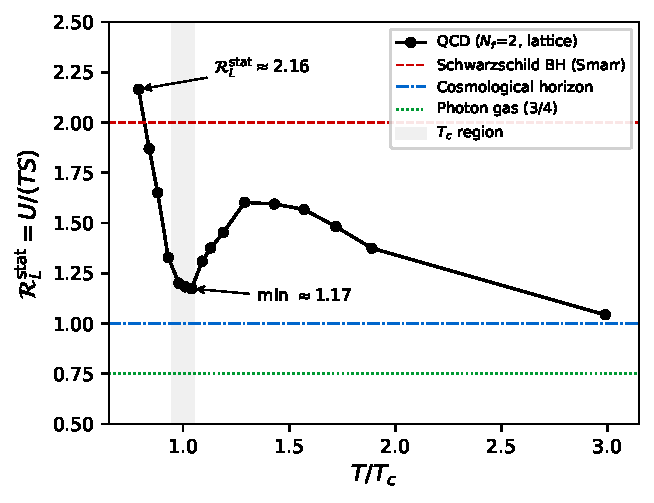
\includegraphics[width=\columnwidth]{fig_rl_qcd.pdf}
\caption{Static Landauer ratio $\RLs = U/(TS)$ for the QCD static
$q\bar{q}$ system as a function of $T/T_c$ (Kaczmarek--Zantow
lattice data, $N_f = 2$, $T_c = 200$~MeV).
Points to the left of the gray band are in the confined (flux-tube)
phase; points to the right are in the deconfined (color-screened)
regime.
Horizontal lines mark the Schwarzschild black hole ($\RLs = 2$,
Smarr relation), cosmological apparent horizon ($\RLs = 1$,
Misner--Sharp; note $\RLd = 1/2$ for this system), and photon gas
($\RLs = 3/4$, Stefan--Boltzmann).}
\label{fig:rl_qcd}
\end{figure}

The free energy $F_{\infty}$ is positive below $T_c$ and decreasing
above $T_c$, consistent with the standard picture: confinement
requires positive free energy (work must be done to separate quarks),
while above $T_c$ color screening reduces the separation cost.

\textbf{Remark (string tension).}
As a dimensional-analysis cross-check, identifying the source strength
of a one-dimensional flux tube with the Landauer cost per bit gives
$\sigma = k_B T_c \ln 2 \cdot \rho_{1D}$, where $\rho_{1D}$ is the
information density along the tube.  Using $\sigma \approx 0.89$~GeV/fm
yields $\rho_{1D} \approx 6.4$~bits/fm (at $T_c = 200$~MeV) or
$\approx 8.3$~bits/fm (at $T_c = 155$~MeV).  Both exceed the bare
color content $\log_2 3 \approx 1.58$~bits, which is expected since
the flux tube also carries gluonic excitations.  This is not a
derivation of $\sigma$ (any ratio of two positive quantities with
the same dimensions yields a positive number), but the result's
consistency with QCD phenomenology is a useful sanity check.

\subsection{Physical interpretation}

The deconfinement transition is the point where the static
$q\bar{q}$ system most closely approaches $\RLs = 1$.  At $T_c$,
the system undergoes a reorganization of its information-storage
structure from one-dimensional (chromoelectric flux tube below
$T_c$, $d=1$) to zero-dimensional (color-screened, quasi-pointlike
charges above $T_c$, $d=0$).

In the $N_f = 2$ dataset, the proximity of QCD deep confinement
($\RLs \approx 2.16$) to the Schwarzschild black hole
($\RLs = 2$) is striking.
Both systems confine information behind a boundary (the horizon for
gravity, the flux tube for color) and both have $U \approx 2\,TS$
in the $N_f = 2$ dataset.  The Smarr
factor of 2 for black holes arises because the Bekenstein--Hawking
entropy scales as $S_{BH} \propto M^2$ (degree~2 in energy), so
Euler's theorem gives $M/T_H = 2\,S_{BH}$, i.e.\ $M = 2\,T_H S_{BH}$;
the QCD factor
$\approx 2$ in deep confinement reflects the analogous energetic
overhead of maintaining the chromoelectric string.
However, convergence near $\RLs = 2$ need not imply a dynamical
link: the Schwarzschild value is fixed by the Euler degree of the
area-law entropy, while the QCD value is a lattice-dependent number
that will shift with $N_f$ and quark masses, so the proximity may be
a coincidence of scaling exponents rather than evidence for a shared
mechanism.

\subsection{Falsifiable conjecture}

The observation that $\RLs > 1$ throughout the confined phase
holds in both the $N_f = 2$ Kaczmarek--Zantow dataset
(Table~\ref{tab:qcd_rl}) and the continuum-extrapolated
(2+1)-flavor Bazavov dataset (Table~\ref{tab:bazavov_rl}),
despite significant differences in lattice setup, quark masses,
and renormalization conventions.  We therefore state the following
as a falsifiable conjecture:

\begin{quote}
\textbf{Conjecture.}
$\RLs > 1$ is a generic thermodynamic signature of confinement
in asymptotically free gauge theories: for any confining gauge
theory (varying gauge group $SU(N)$, number of flavors $N_f$,
and quark masses), the static Landauer ratio satisfies
$\RLs > 1$ in the confined phase and reaches a minimum near
the deconfinement transition temperature $T_c$.
\end{quote}

This conjecture is testable by computing $\RLs$ from existing
or future lattice data for:
\begin{enumerate}
\item Pure $SU(N)$ gauge theories at $N = 2, 3, 4, 5$ (where the
deconfinement transition sharpens with increasing $N$);
\item $SU(3)$ with varying $N_f$ and quark masses (to separate
the effects of light-quark screening from confinement);
\item $Sp(N)$ and $G_2$ gauge theories (to test universality
beyond $SU(N)$).
\end{enumerate}
A single counterexample---a confining gauge theory exhibiting
$\RLs < 1$ in the confined phase---would falsify the conjecture.
Conversely, if the conjecture holds, the minimum of $\RLs(T)$
would provide a thermodynamic marker for the deconfinement
crossover, complementary to the Polyakov loop order parameter.

\textbf{Important caveat.} The conjecture is specifically that
$\RLs > 1$ is a \emph{necessary} thermodynamic feature of the
confined phase, not that it is \emph{sufficient} for confinement.
The lattice data show $\RLs > 1$ persisting well above $T_c$
(e.g., $\RLs = 1.04$ at $T/T_c = 2.99$ in the deconfined,
color-screened regime).  Thus $\RLs > 1$ alone does not
discriminate confined from deconfined phases; rather, the
conjecture is that $\RLs < 1$ would rule out confinement.


% ============================================================
\section{Thermal Casimir effect: \texorpdfstring{$\RLs$}{RL} in the entropic regime}
\label{sec:casimir}

\subsection{Setup}

The Casimir free energy per unit area between two perfectly conducting
plates separated by distance $a$ at temperature $T$ interpolates
between a quantum regime ($\tau \ll 1$) and a classical regime
($\tau \gg 1$), where the dimensionless temperature is
\begin{equation}
\tau \equiv \frac{2\pi a k_B T}{\hbar c}.
\end{equation}

\subsection{Zero-temperature limit}

At $T = 0$, the Casimir energy is purely quantum mechanical:
\begin{equation}
\frac{F_0}{A} = -\frac{\pi^2 \hbar c}{720\, a^3}.
\end{equation}
The entropy vanishes ($S = 0$), so $F = U = F_0$ and $\RLs$
is undefined (no information content to erase).

\subsection{High-temperature (classical) limit}

For $\tau \gg 1$, the free energy becomes~\cite{Lifshitz1956}
\begin{equation}
\frac{F}{A} \to -\frac{\zeta(3)\, k_B T}{8\pi a^2},
\end{equation}
which is purely linear in $T$.  The entropy per unit area is
\begin{equation}
\frac{S}{A} = -\frac{1}{A}\frac{\partial F}{\partial T}
= \frac{\zeta(3)\, k_B}{8\pi a^2},
\end{equation}
and the internal energy is
\begin{equation}
\frac{U}{A} = \frac{F}{A} + T\frac{S}{A} = 0.
\end{equation}

The Casimir free energy in the high-$T$ limit is \emph{entirely
entropic}: $F = -TS$, $U = 0$.  The static Landauer ratio is
therefore
\begin{equation}
\mathcal{R}_L^{\mathrm{Casimir}} = \frac{U}{T S} \to 0
\qquad (\tau \gg 1).
\end{equation}

\subsection{Interpretation}

The thermal Casimir effect is \emph{sub-Landauer}: the static
energy-to-information ratio falls below unity.  In this limit, the
Casimir \emph{interaction} contribution to the internal energy
vanishes; the entire interaction free energy arises from the entropy
of suppressed electromagnetic modes between the plates.  (The total
internal energy of the electromagnetic field is of course nonzero;
what vanishes is the boundary-dependent part.)

This makes the Casimir effect the thermodynamic opposite of QCD
confinement and black holes:
\begin{itemize}
\item \textbf{QCD and BH}: $\RLs > 1$.  Internal
energy dominates; these confining systems have $U > TS$.
\item \textbf{Casimir}: $\RLs \to 0$.  Entropy dominates.
The interaction force is driven purely by the entropic cost of
boundary conditions, with no interaction internal energy.
\end{itemize}

The crossover from quantum ($U$-dominated) to classical
($S$-dominated) Casimir behavior occurs at $\tau \sim 1$, i.e.,
\begin{equation}
T_{\mathrm{cross}} = \frac{\hbar c}{2\pi a k_B}.
\end{equation}
For plate separation $a = 1~\mu\mathrm{m}$, $T_{\mathrm{cross}} \approx 365$~K.
As the system crosses from quantum to classical, $\RLs$
decreases toward zero; the detailed trajectory depends on the
sign conventions for Casimir internal energy and is left to
future dedicated analysis.


% ============================================================
\section{Unified classification}
\label{sec:classification}

Table~\ref{tab:classification} collects the static $\RLs$
values across all systems studied in Papers~C and~D, together with
two benchmark systems (photon gas, cosmological horizon) that
anchor the classification.

\begin{table}[t]
\centering
\caption{Static Landauer ratio $\RLs = U/(TS)$ across
physical systems.  QCD values from Kaczmarek--Zantow
($N_f = 2$, $T_c = 200$~MeV); see Table~\ref{tab:bazavov_rl}
for (2+1)-flavor results.  Photon gas: $U = aVT^4$,
$S = \tfrac{4}{3}aVT^3$, so $TS = \tfrac{4}{3}U$ and
$\RLs = 3/4$.
$^{\dagger}$This point is in the deconfined (color-screened)
regime; $\RLs > 1$ here does not indicate confinement
(see Section~\ref{sec:perturbative}).
$^{\ddagger}$Static ratio only; the differential ratio from
Paper~C gives $\RLd = 1/2$ for this system.}
\label{tab:classification}
\begin{tabular}{@{}llll@{}}
\toprule
System & $\RLs$ & Regime & Source \\
\midrule
QCD, deep confinement & 2.16 & Super & KZ, $N_f\!=\!2$ \\
Schwarzschild BH      & 2    & Super & Smarr \\
QCD, at $T_c$         & 1.17 & Super & KZ, $N_f\!=\!2$ \\
QCD, $T/T_c = 2.99$ (deconfined) & 1.04 & Super$^{\dagger}$ & KZ, $N_f\!=\!2$ \\
\midrule
Cosmological apparent horizon & 1 & Saturating$^{\ddagger}$ & Misner--Sharp \\
\midrule
Photon gas (blackbody) & 3/4  & Sub & Stefan--Boltzmann \\
Casimir, high-$T$      & 0    & Sub & Exact \\
\bottomrule
\end{tabular}
\end{table}

The classification has three regimes:

\begin{enumerate}
\item \textbf{Super-Landauer} ($\RLs > 1$): Systems that
confine information behind a boundary.  Both the Schwarzschild black
hole ($\RLs = 2$, exact) and QCD deep confinement
($\RLs \approx 2$--$3$ depending on lattice setup) fall in this
regime.  Despite the vastly different physical scales, both systems
share the structural feature $U > TS$.

\item \textbf{Statically saturating} ($\RLs = 1$):
The cosmological apparent horizon, where the Misner--Sharp energy
exactly equals the entropy-weighted temperature.  Note that the
\emph{differential} ratio from Paper~C gives $\RLd = 1/2$ for
this system; the label ``saturating'' applies only to the static
ratio and should not be conflated with the process-level diagnostic.

\item \textbf{Sub-Landauer} ($\RLs < 1$): Systems where $U < TS$,
i.e., the entropy contribution to the free energy exceeds the
internal energy.  The label ``sub-Landauer'' refers to the static
energy-to-information ratio, not to any violation of Landauer's
erasure bound (which constrains processes, not static states).
The photon gas provides a clean benchmark: $U \propto T^4$ and
$S \propto T^3$ give $TS = (4/3)U$, hence $\RLs = 3/4$ exactly.
The high-$T$ Casimir effect reaches the extreme $\RLs = 0$
(purely entropic interaction free energy, no interaction internal
energy).
\end{enumerate}

\subsection{Relation to Paper~C}

Paper~C~\cite{Rahnama2026BlackHole} defined a \emph{differential}
Landauer ratio $\mathcal{R}_L^{\mathrm{diff}} = \delta E/(T\,\delta S)$
for thermodynamic processes at horizons.  The differential ratio gives
$\mathcal{R}_L^{\mathrm{diff}} = 1$ for black hole evaporation
(from the first law $dM = T_H\,dS_{BH}$) and
$\mathcal{R}_L^{\mathrm{diff}} = 1/2$ for the cosmological apparent
horizon (from Trivedi's quasi-local energy
accounting~\cite{Trivedi2024}).

The static ratio defined here, $\RLs = U/(TS)$, measures a
different quantity: the total energy budget relative to total
information content, rather than the marginal cost per bit during a
process.  For systems with homogeneous entropy, the two are related
by $\RLs = n \times \RLd$, where $n$ is the Euler degree.  For
Schwarzschild, $S_{BH} \propto M^2$ gives $n = 2$, so
$\RLs = 2 \times 1 = 2$.  The cosmological apparent horizon
gives $\RLs = 1$ directly from $E_{MS} = T_{\mathrm{GH}}\,S$
(Misner--Sharp accounting).  The Euler-degree decomposition
does not straightforwardly apply here: the area--energy relation
gives $S \propto E_{MS}^2$ (as for black holes), but the
Gibbons--Hawking temperature $T_{\mathrm{GH}} = \hbar H/(2\pi k_B)$
differs from $(\partial S/\partial E_{MS})^{-1}$ by a factor of~2,
so $\RLs = 1$ is an algebraic consequence of the Misner--Sharp
bookkeeping rather than a simple Euler-degree statement.

Both definitions are valid diagnostics.  The differential ratio is
natural for dynamic processes (evaporation, expansion); the static
ratio is natural for comparing equilibrium systems (QCD, Casimir)
where no process is involved.


% ============================================================
\section{Perturbative high-temperature limit}
\label{sec:perturbative}

At asymptotically high temperatures, QCD perturbation theory
controls the static $q\bar{q}$ free energy through the Polyakov
loop correlator.  The leading contribution to $F_{\infty}$ is
$\sim g^2 T$ (one-gluon exchange with Debye screening),
with higher-order corrections at $g^3$, $g^4\ln g$,
etc.~\cite{Linde1980,BraatenNieto1996,KZ2005a}.
Because the entropy $S_{\infty} = -\partial F_{\infty}/\partial T$
inherits terms from the running of $g(T)$, and because
asymptotic freedom drives $g \to 0$ as $T \to \infty$,
$\RLs = U_{\infty}/(T\,S_{\infty})$ vanishes
in this limit:
\begin{equation}
\mathcal{R}_L^{\mathrm{QCD}}(T)
\xrightarrow{T \to \infty} 0.
\end{equation}
The precise functional form of the approach to zero (e.g.,
$\sim g^2(T)$) depends on the detailed perturbative structure
of $F_{\infty}(T)$ and is left to future work.

This means the QCD $\RLs$ must cross through unity at some
temperature above $T_c$.  The lattice data show
$\RLs = 1.04$ at $T/T_c = 2.99$, so the crossing
$\RLs = 1$ occurs at $T/T_c \gtrsim 3$.

The physical picture is clear: at very high temperatures, the static
$q\bar{q}$ system transitions from a super-Landauer confined regime
(flux tube below $T_c$, storing excess energy) through a
still-super-Landauer near-$T_c$ region to a sub-Landauer screened
regime (color-screened charges with entropy-dominated free energy),
crossing $\RLs = 1$ at $T/T_c \gtrsim 3$.  This
mirrors the Casimir quantum-to-classical crossover, where
$\RLs$ also decreases from above to below unity as
thermal effects dominate.


% ============================================================
\section{Cross-consistency with Papers~A, B, and C}

The results of this paper are consistent with the trilogy framework:

\begin{enumerate}
\item \textbf{Paper~A}~\cite{Rahnama2026A}: Paper~A derives a
conditional record-formation heat bound
$Q \geq k_B T \ln 2 \cdot I(X;Y)$ for quantum measurement under
explicit operational conditions (C1 to C6).  The denominator of
$\RLs$ can be written as $TS = N_{\mathrm{bits}}\,k_B T \ln 2$,
which admits a Landauer interpretation as the total maintenance cost
of the system's information content; however, $\RLs$ itself is a
standard thermodynamic quantity (the Euler homogeneity degree) and
does not require Paper~A's process-level bound for its definition
or computation.

\item \textbf{Paper~B}~\cite{Rahnama2026BornRule}: The Born rule
$p_i = |\alpha_i|^2$ is derived as the unique probability rule
consistent with normalization, phase independence, tensor-product
factorization, and continuity under record-formation constraints.
$\RLs$ provides a complementary static diagnostic: it measures
the energy-to-information ratio in the system's thermodynamic
bookkeeping.

\item \textbf{Paper~C}~\cite{Rahnama2026BlackHole}: The differential
$\RLd$ diagnostic is defined for gravitational horizons.
The present paper extends the analysis to non-gravitational
systems using the static ratio, and relates the two definitions
through the Smarr homogeneity factor
(Section~\ref{sec:classification}).

\item \textbf{Smarr relation}: The static $\RLs = 2$ for black
holes follows from the Smarr relation ($Mc^2 = 2T_H S_{BH}$),
connecting the differential ratio of Paper~C to the static ratio
used here via the Euler homogeneity factor.
\end{enumerate}


% ============================================================
\section{Scope: what this paper does and does not claim}
\label{sec:scope}

\textbf{What we claim:}
\begin{enumerate}
\item The static Landauer ratio $\RLs = U/(TS)$ is a useful
diagnostic for comparing the energy budgets of thermodynamic systems.
\item The QCD static $q\bar{q}$ system is super-Landauer
($\RLs > 1$) throughout the confined phase and near-$T_c$
region, with deep-confinement values of
$\RLs \approx 2$--$3$ (depending on lattice setup) and a
minimum near $T_c$.  The ratio remains above unity into the
deconfined regime up to $T/T_c \approx 3$, crossing to
sub-Landauer at asymptotically high temperatures.
\item The high-$T$ Casimir effect is sub-Landauer
($\RLs \to 0$), computed from exact analytical results.
\item The geometric-scaling correspondence between storage
dimension and force law ($F \sim r^{d-1}$ for $d \geq 1$;
$F \sim 1/r^2$ for $d = 0$) admits a Landauer
interpretation but is not derived from information theory.
\item The implied flux-tube information density ($6$--$8$~bits/fm) is
a dimensional-analysis cross-check consistent with QCD phenomenology
(see the remark in Section~\ref{sec:qcd}).
\item The super-Landauer pattern ($\RLs > 1$ in confinement,
minimum at $T_c$) is confirmed independently by (2+1)-flavor
continuum-extrapolated lattice data~\cite{Bazavov2016}
(Table~\ref{tab:bazavov_rl}).
\item We conjecture that $\RLs > 1$ is a generic thermodynamic
signature of confinement in asymptotically free gauge theories,
falsifiable by computing $\RLs$ across gauge groups and flavor
content (Section~\ref{sec:qcd}).
\end{enumerate}

\textbf{What we do not claim:}
\begin{enumerate}
\item We do not derive coupling constants, the QCD string tension,
or the fine structure constant from the Landauer framework.
\item We do not modify QCD, QED, or general relativity.
\item We do not claim that information storage ``causes'' forces.
The storage-dimension correspondence (Section~\ref{sec:storage_dim})
follows from geometric scaling; the Landauer framing provides a
thermodynamic interpretation but no dynamical mechanism.
\item We do not claim that the near-coincidence
$\mathcal{R}_L^{\mathrm{QCD}} \approx \mathcal{R}_L^{\mathrm{BH}}
\approx 2$ implies a dynamical connection between QCD confinement
and gravity.  It is a thermodynamic observation that may or may not
have deeper significance.
\item The Kaczmarek--Zantow data use $N_f = 2$ with heavier-than-physical
quark masses.  The qualitative features (minimum at $T_c$,
$\RLs > 1$) persist in the (2+1)-flavor Bazavov data with
physical quark masses (Table~\ref{tab:bazavov_rl}), but the
precise $\RLs$ values differ due to different renormalization
conventions and lattice setups.
\end{enumerate}


% ============================================================
\section{Conclusion}
\label{sec:conclusion}

We have defined the static Landauer ratio $\RLs = U/(TS)$
and computed it for QCD static-quark thermodynamics and the thermal
Casimir effect.
Combined with gravitational systems, the results define a
three-regime classification:

\begin{enumerate}
\item \textbf{Super-Landauer} ($\RLs > 1$):
Schwarzschild black holes ($\RLs = 2$, exact via Smarr) and
QCD deep confinement ($\RLs \approx 2$--$3$ depending on
lattice setup).  Both systems confine information behind a boundary
and store well above the $\RLs = 1$ threshold.  Note that the
static $q\bar{q}$ system remains super-Landauer into the
deconfined regime up to $T/T_c \approx 3$; the conjecture that
$\RLs > 1$ is a confinement signature applies specifically to
the confined phase ($T < T_c$).

\item \textbf{Statically saturating} ($\RLs = 1$):
The cosmological apparent horizon, where the Misner--Sharp energy
exactly equals the entropy-weighted temperature.  (The differential
ratio from Paper~C gives $\RLd = 1/2$ for this system.)

\item \textbf{Sub-Landauer} ($\RLs < 1$):
The photon gas ($\RLs = 3/4$, exact), high-temperature
Casimir ($\RLs \to 0$), and at asymptotically high
temperatures, the screened QCD regime
($\RLs \to 0$ by asymptotic freedom).
\end{enumerate}

The headline result is that black holes and QCD in the confined phase
are both robustly super-Landauer ($\RLs > 1$), despite operating at
vastly different scales.  Both systems confine information behind a
boundary and both satisfy $U > TS$, placing them well above the
$\RLs = 1$ threshold.

The companion simulation verifies the numerical claims from the
Kaczmarek--Zantow static-quark dataset and all derived quantities
through 80 falsifiable checks across 9 groups, including negative
tests that confirm wrong inputs produce wrong outputs.  The Bazavov
(2+1)-flavor values in Table~\ref{tab:bazavov_rl} are computed
directly from the continuum-extrapolated data in
Ref.~\cite{Bazavov2016} (Table~XIII therein).

\section*{Code Availability}
The supplementary simulation code and generated consistency reports
are available at
\url{https://github.com/MosesRahnama/paper-d-landauer-beyond-horizons}.

\begin{thebibliography}{99}

\bibitem{Landauer1961}
R.~Landauer, ``Irreversibility and Heat Generation in the Computing
Process,''
IBM J.\ Res.\ Dev.\ \textbf{5}, 183 (1961).

\bibitem{Cortes2024}
M.~Cort\^es and A.~R.~Liddle, ``Hawking evaporation and the
Landauer Principle,''
arXiv:2407.08777 [gr-qc] (2024).

\bibitem{Rahnama2026BlackHole}
M.~Rahnama, ``Black Holes as Landauer-Saturating Erasure Channels:
Horizon Diagnostics, Area Quantization, and the Measurement
Complement,''
Preprints (2026), submitted.

\bibitem{Trivedi2024}
A.~Trivedi, ``Landauer's principle and information at the
cosmological horizon,''
arXiv:2407.15231v3 (2024).

\bibitem{Smarr1973}
L.~Smarr, ``Mass Formula for Kerr Black Holes,''
Phys.\ Rev.\ Lett.\ \textbf{30}, 71 (1973).

\bibitem{KZ2005a}
O.~Kaczmarek and F.~Zantow, ``Static quark--antiquark interactions
at zero and finite temperature QCD.\ II.\ Quark--antiquark internal
energy and entropy,''
arXiv:hep-lat/0506019 (2005).

\bibitem{KZ2005b}
O.~Kaczmarek and F.~Zantow, ``Static quark--antiquark interactions
in zero and finite temperature QCD.\ I.\ Heavy quark free energies,
running coupling, and quarkonium binding,''
Phys.\ Rev.\ D \textbf{71}, 114510 (2005),
arXiv:hep-lat/0503017.

\bibitem{Casimir1948}
H.~B.~G.~Casimir, ``On the attraction between two perfectly
conducting plates,''
Proc.\ K.\ Ned.\ Akad.\ Wet.\ \textbf{51}, 793 (1948).

\bibitem{Lifshitz1956}
E.~M.~Lifshitz, ``The theory of molecular attractive forces between
solids,''
Sov.\ Phys.\ JETP \textbf{2}, 73 (1956).

\bibitem{BraatenNieto1996}
E.~Braaten and A.~Nieto, ``Free energy of QCD at high temperature,''
Phys.\ Rev.\ D \textbf{53}, 3421 (1996),
arXiv:hep-ph/9510408.

\bibitem{Bazavov2016}
A.~Bazavov, N.~Brambilla, H.-T.~Ding, P.~Petreczky,
H.-P.~Schadler, A.~Vairo, and J.~H.~Weber,
``Polyakov loop in 2+1 flavor QCD from low to high temperatures,''
Phys.\ Rev.\ D \textbf{93}, 114502 (2016),
arXiv:1603.06637.

\bibitem{Linde1980}
A.~D.~Linde, ``Infrared problem in the thermodynamics of the
Yang--Mills gas,''
Phys.\ Lett.\ B \textbf{96}, 289 (1980).

\bibitem{Rahnama2026A}
M.~Rahnama, ``Calorimetric Signature of Quantum Measurement: A
Record-Formation Heat Bound and Differential Microcalorimetry Test,''
Preprints \textbf{2026}, 202602.1739 (2026).
\url{https://doi.org/10.20944/preprints202602.1739.v2}.

\bibitem{Rahnama2026BornRule}
M.~Rahnama, ``Born's Rule from Record-Formation Constraints: A
Thermodynamic-Information Axiomatics,''
Preprints \textbf{2026}, 202603.0473 (2026).
\url{https://doi.org/10.20944/preprints202603.0473.v1}.

\bibitem{Callen1985}
H.~B.~Callen, \emph{Thermodynamics and an Introduction to
Thermostatistics}, 2nd ed.\ (Wiley, New York, 1985),
Ch.~3 (Euler relation and homogeneous functions).

\bibitem{KastorRayTraschen2009}
D.~Kastor, S.~Ray, and J.~Traschen, ``Enthalpy and the mechanics
of AdS black holes,''
Class.\ Quantum Grav.\ \textbf{26}, 195011 (2009),
arXiv:0904.2765.

\end{thebibliography}

\end{document}
